\documentclass[12pt,a4paper,twoside]{article} % 启用双面模式
\usepackage[UTF8]{ctex} % 中文支持
\usepackage{geometry} % 页面布局
\usepackage{multicol} % 分栏布局
\usepackage{setspace} % 行间距
\usepackage{fancyhdr} % 页眉页脚设置
\usepackage{titlesec} % 调整标题间距
\usepackage{enumitem} % 控制列表间距
\usepackage{fontspec} % 字体支持
\usepackage{lipsum} % 占位文本
\usepackage{amsmath} 
\usepackage{graphicx}
\usepackage{float}
\restylefloat{figure}
\usepackage{caption}
\usepackage{amssymb}
\usepackage{natbib}

% 使用 Times New Roman 字体
\setmainfont{Times New Roman} % 设置主字体为 Times New Roman

\bibliographystyle{plain}

% 定义统一页面布局(适用于所有页面)
\geometry{
    a4paper,
    top=1in,
    bottom=0.8in,       % 统一底边距
    left=0.35in,
    right=0.35in,
    footskip=0in    % 统一页脚跳距
}

% 行距和缩进
\renewcommand{\baselinestretch}{1.3} % 行距1.3倍
\setlength{\parindent}{1em}         % 段落缩进2em

% 定义带空格的标题
\newcommand{\universityjournal}{北\hspace{0.5em}京\hspace{0.5em}邮\hspace{0.5em}电\hspace{0.5em}大\hspace{0.5em}学\hspace{0.5em}学\hspace{0.5em}报}

% 设置标题自动显示到页眉(用于动态更新奇数页的标题)
\makeatletter
\newcommand{\articleauthor}{王语兰} % 作者名
\newcommand{\articletitle}{参数高效微调方法研究及其在计算机视觉中的应用} % 默认文章标题
\renewcommand{\sectionmark}[1]{\markboth{\articleauthor: #1}{}}
\makeatother

% 首页页眉页脚样式
\fancypagestyle{firstpage}{
    \fancyhf{} % 清空默认页眉页脚
    \renewcommand{\headrule}{% 自定义双横线
        \vspace{0.5ex}
        \hrule height 0.5pt
        \vspace{0.5ex}
        \hrule height 0.5pt
        \vspace{-1.5ex}
    }
    % 左侧页眉
    \fancyhead[L]{2025 年 1 月 \\ 第 xx 卷 第 x 期}
    % 中间页眉
    \fancyhead[C]{\universityjournal \\ Journal of Beijing University of Posts and Telecommunications}
    % 右侧页眉
    \fancyhead[R]{Jan. 2025 \\ Vol. xx No. x}
    
    % 保留现有首页页脚设置
    \fancyfoot[L]{%
        \rule[0pt]{0.3\textwidth}{0.4pt}\\ % 页脚上方短横线
        % \vspace{-3em} % 向上移动页脚内容
        \scriptsize % 减小字体到小五号
        \textbf{收稿日期:} 2025-01-05 \\ % 四行信息靠左对齐
        \textbf{基金项目:} 无 \\
        \textbf{作者简介:} 王语兰(2002—),女,学号2020211240,研究方向为深度学习。 \\
        \textbf{通信作者:} 王语兰,邮箱:wangyulan@bupt.edu.cn。
    }
}

% 正文页眉页脚样式
\pagestyle{fancy}
\fancyhf{} % 清空默认设置

% 正文页头的单横线
\renewcommand{\headrulewidth}{0.5pt} % 正文单横线

% 奇数页设置
\fancyhead[LO]{第 x 期} % 奇数页左侧
\fancyhead[CO]{\articleauthor: \articletitle} % 奇数页中间
\fancyhead[RO]{\thepage} % 奇数页右侧页码

% 偶数页设置
\fancyhead[LE]{\thepage} % 偶数页左侧页码
\fancyhead[CE]{\universityjournal} % 偶数页中间
\fancyhead[RE]{第 xx 卷} % 偶数页右侧

% 清空页脚,确保后续页面无页脚
\fancyfoot{} 

% 段间距与行距
\setlength{\parskip}{0pt}         % 段间距设为 0
\renewcommand{\baselinestretch}{1.2} % 行间距设为 1.0

% 标题间距调整
\titlespacing*{\section}{0pt}{0pt}{0pt}    % section 无段前段后间距
\titlespacing*{\subsection}{0pt}{0pt}{0pt} % subsection 无段前段后间距
\titlespacing*{\subsubsection}{0pt}{0pt}{0pt}
\titlespacing*{\paragraph}{0pt}{0pt}{*}

% 公式间距调整
\makeatletter
\g@addto@macro\normalsize{%
    \setlength{\abovedisplayskip}{0pt}%
    \setlength{\belowdisplayskip}{0pt}%
    \setlength{\abovedisplayshortskip}{0pt}%
    \setlength{\belowdisplayshortskip}{0pt}%
}
\makeatother

% 列表间距调整
\usepackage{enumitem} % 列表格式控制
\setlist[itemize]{itemsep=0pt, topsep=0pt, parsep=0pt, partopsep=0pt}
\setlist[enumerate]{itemsep=0pt, topsep=0pt, parsep=0pt, partopsep=0pt}

\setlength{\intextsep}{0pt}
\captionsetup[figure]{skip=0pt} % 设置图片与图注之间的距离为 0pt

\setlength{\columnsep}{1cm} % 设置两栏之间的距离为 1cm

\setlength{\bibsep}{0pt}
\begin{document}

% 1. 应用首页页眉页脚样式
\thispagestyle{firstpage}

% 2. 首页内容
% 文章编号与 DOI
\noindent
\textbf{文章编号:} xxxx-xxxx(2025)xx-xxxx-xx \hspace{1cm} \textbf{DOI:} xx.xxxxx/j.jbupt.2025-xxx \\[0.8em]

% 中文标题
\begin{center}
    {\LARGE \textbf{参数高效微调方法研究及其在计算机视觉中的应用}}
\end{center}

% 中文作者
\begin{center}
    {\large 王语兰}\\[0.1em]
    {\footnotesize
    (北京邮电大学 计算机科学与技术学院(国家示范性软件学院), 北京 100876)
    }
\end{center}

% 中文摘要
\noindent
\textbf{摘要:} 本文系统地研究了基于深度学习的参数高效微调(PEFT)方法,旨在在降低计算和存储成本的同时,保持或提升预训练模型在下游任务中的性能。本文首先分类讨论了增量式微调、选择性微调和参数重构微调三类主要PEFT方法,并详细分析了它们的原理和应用。随后,本文探讨了PEFT方法在计算机视觉领域的具体应用,包括视觉变换器(ViTs)和视觉-语言对齐模型(VLAs)。最后,本文总结了PEFT领域的未来研究方向和挑战,如简化超参数调整、建立统一基准、提升训练效率等。实验结果表明,PEFT方法在多种任务中表现出色,展示了其在实际应用中的潜力。

% 中文关键词
\noindent
\textbf{关\hspace{0.5em}键\hspace{0.5em}词:} 参数高效微调;深度学习;计算机视觉;预训练模型;模型适配

% 中图分类号与文献标志码
\noindent
\textbf{中图分类号:} TP393.0 \hspace{3em} \textbf{文献标志码:} A

% 英文标题
\begin{center}
    {\Large \textbf{Research on Parameter-Efficient Fine-Tuning Methods Based on Deep Learning and Their Applications in Computer Vision}}
\end{center}

% 英文作者
\begin{center}
    {\large WANG Yulan}\\[0.1em]
    {\footnotesize
    (School of Computer Science (National Pilot Software Engineering School), Beijing University of Posts and Telecommunications, Beijing 100876, China)
    }
\end{center}

% 英文摘要
\noindent
\textbf{Abstract:} This paper systematically investigates parameter-efficient fine-tuning (PEFT) methods based on deep learning, aiming to reduce computational and storage costs while maintaining or enhancing the performance of pre-trained models on downstream tasks. The paper first categorizes the three main PEFT approaches: additive fine-tuning, selective fine-tuning, and reparameterized fine-tuning, providing detailed analyses of their principles and applications. Subsequently, the application of PEFT methods in the field of computer vision is explored, including their use in Vision Transformers (ViTs) and Vision-Language Alignment models (VLAs). Finally, the paper summarizes future research directions and challenges in the PEFT domain, such as simplifying hyperparameter tuning, establishing unified benchmarks, and improving training efficiency. Experimental results demonstrate that PEFT methods perform excellently across various tasks, highlighting their potential in practical applications.

% 英文关键词
\noindent
\textbf{Key words:} Parameter-Efficient Fine-Tuning; Deep Learning; Computer Vision; Pre-trained Models; Model Adaptation


% 正文填充(模拟较大底边距)
% \vspace{1em} % 增加必要的间距

% 正文开始
\begin{multicols}{2}
\noindent
\section{引言}

随着深度学习技术的迅猛发展,预训练模型在自然语言处理、计算机视觉等多个领域取得了显著的成果。然而,这些预训练模型通常拥有数亿甚至数十亿的参数,导致在实际应用中面临高昂的计算和存储成本。尤其是在资源受限的环境下,如何高效地适配预训练模型以应对不同的下游任务,成为研究的热点问题。

参数高效微调(Parameter-Efficient Fine-Tuning, PEFT)方法应运而生,旨在通过仅调整模型的一小部分参数,显著降低微调过程中的计算开销和存储需求,同时保持或提升模型在目标任务上的性能。与传统的全参数微调方法相比,PEFT 方法不仅提高了训练效率,还在多任务学习和模型部署等场景中展现出更强的灵活性和适应性。

本综述系统地回顾了基于深度学习的参数高效微调方法,首先对现有的主要 PEFT 方法进行了分类和原理分析,包括增量式微调、选择性微调和参数重构微调。随后,重点探讨了这些方法在计算机视觉领域中的具体应用,如视觉变换器(Vision Transformers, ViTs)和视觉-语言对齐模型(Vision-Language Alignment models, VLAs)的微调策略。最后,总结了当前 PEFT 研究面临的挑战,并展望了未来的发展方向。

通过对 PEFT 方法的深入分析和应用探讨,本文旨在为研究人员和工程师提供一个全面的参考,促进参数高效微调技术在各类深度学习应用中的进一步发展和普及。

\section{参数高效微调方法分类及其原理}

参数高效微调(Parameter-Efficient Fine-Tuning, PEFT)是一种通过减少模型微调参数数量来降低计算成本和存储需求的方法。PEFT 方法被广泛应用于大规模预训练模型,其主要目标是高效适配下游任务,同时最大程度保留预训练模型的知识。根据微调过程中参数的调整方式和设计思路,PEFT 方法可以分为以下三类:


\subsection{增量式微调(Additive Fine-Tuning)}
增量式微调通过在预训练模型的基础上引入少量新增参数来实现任务适配。新增模块通常以瓶颈结构呈现,即先通过降维矩阵 $\mathbf{W}_{\text{down}}$ 将输入特征降至较小的维度,再通过升维矩阵 $\mathbf{W}_{\text{up}}$ 恢复至原始维度,公式如下:
\begin{equation}
\mathbf{h}_{\text{out}} = \mathbf{W}_0 \mathbf{h}_{\text{in}} + \alpha \mathbf{W}_{\text{up}} \sigma (\mathbf{W}_{\text{down}} \mathbf{h}_{\text{in}}),
\label{eq:additive}
\end{equation}
其中,$\mathbf{W}_0$ 为冻结的预训练参数,$\mathbf{W}_{\text{up}}$ 和 $\mathbf{W}_{\text{down}}$ 为新增可训练参数,$\alpha$ 为缩放因子,$\sigma(\cdot)$ 为非线性激活函数(如 ReLU)。该方法通过引入适配器或提示向量等模块,灵活适配多种任务需求。

\subsection{选择性微调(Selective Fine-Tuning)}
选择性微调通过冻结大部分模型参数,仅对一部分重要参数进行优化。这种方法依赖于参数重要性评估策略,如 Fisher 信息矩阵或梯度幅度筛选,挑选对任务影响最大的参数进行训练。其数学描述如下:
\begin{equation}
\theta_i' = \theta_i - \eta m_i \frac{\partial \mathcal{L}}{\partial \theta_i},
\label{eq:selective}
\end{equation}
其中,$\theta_i$ 为原始模型参数,$\mathcal{L}$ 为损失函数,$\eta$ 为学习率,$m_i \in \{0, 1\}$ 是掩码变量,决定参数 $\theta_i$ 是否更新。选择性微调可以采用无结构掩码(逐参数选择)或结构化掩码(对特定层或模块分组选择)的方式。

\begin{figure}[H]
    \centering
    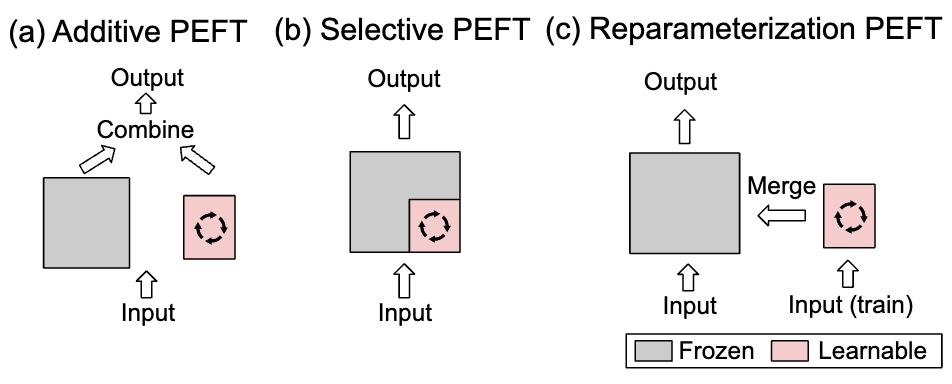
\includegraphics[width=\linewidth]{img/categorize.png}
    \caption{不同类型的 PEFT 算法}
    \label{fig:categorize}
\end{figure}

\subsection{参数重构微调(Reparameterized Fine-Tuning)}
参数重构微调通过重新表征模型的参数,采用低秩分解等技术减少微调的参数量。假设权重矩阵 $\mathbf{W}_0$ 被分解为低秩矩阵 $\mathbf{W}_{\text{up}}$ 和 $\mathbf{W}_{\text{down}}$,其更新公式为:
\begin{equation}
\mathbf{W} = \mathbf{W}_0 + \mathbf{W}_{\text{up}} \mathbf{W}_{\text{down}},
\label{eq:reparameterized}
\end{equation}
其中,$\mathbf{W}_{\text{up}}$ 和 $\mathbf{W}_{\text{down}}$ 是可训练参数,通常满足 $r \\ll \min(d, k)$($r$ 为低秩矩阵的秩)。这种方法通过减少参数的冗余性,实现计算和存储的优化。

\subsection{小结}
上述三类方法各有特点。增量式微调注重模块化设计,适配灵活;选择性微调通过参数筛选实现精简优化;参数重构微调则通过低秩设计在高效性上表现出色。它们共同构成了 PEFT 方法的重要框架,为下游任务提供了多样化的解决方案。


\section{代表性算法}

参数高效微调(Parameter-Efficient Fine-Tuning, PEFT)旨在减少大规模预训练模型在任务适配过程中的计算和存储开销,同时保持或提升模型性能。根据微调过程中对参数的调整方式,PEFT 方法可以分为以下三类:增量式微调、选择性微调和参数重构微调。


\subsection{增量式微调(Additive Fine-Tuning)}

增量式微调是一种通过在预训练模型基础上引入少量可训练参数的技术。这些新增参数以模块化的方式嵌入到模型的不同位置,而预训练的主干网络参数保持冻结不变,仅对新增参数进行优化。这种方法显著减少了需要更新的参数数量,同时能够高效适配新的下游任务 \cite{han2024peft}。

\subsubsection{基本原理}
增量式微调的核心思想是利用少量新增参数对模型的行为进行调整,而不改变主干模型的整体结构。假设预训练模型的参数表示为 $\mathbf{W}_0$,输入为 $\mathbf{h}_{\text{in}}$,输出为 $\mathbf{h}_{\text{out}}$,则增量式微调的计算公式如下:
\begin{equation}
\mathbf{h}_{\text{out}} = \mathbf{W}_0 \mathbf{h}_{\text{in}} + \alpha \mathbf{W}_{\text{up}} \sigma(\mathbf{W}_{\text{down}} \mathbf{h}_{\text{in}}),
\label{eq:additive}
\end{equation}
其中 $\mathbf{W}_0$ 是冻结的预训练模型参数,$\mathbf{W}_{\text{up}}$ 和 $\mathbf{W}_{\text{down}}$ 分别表示上采样矩阵和下采样矩阵,$\alpha$ 是用于调节新增模块影响的缩放因子,$\sigma(\cdot)$ 是非线性激活函数(例如 ReLU)。新增模块的设计通常采用瓶颈结构,即 $\mathbf{W}_{\text{down}}$ 将输入特征降维到较小的维度,$\mathbf{W}_{\text{up}}$ 再将其还原回原始维度。这种设计能够显著降低计算成本和参数数量 \cite{adapter2021}。

\subsubsection{适配器模块(Adapter)}
适配器是增量式微调最常见的方法之一。其基本思想是在每个 Transformer 层中插入一个轻量级的适配器模块,该模块仅增加少量可训练参数,同时保持模型的主干参数冻结。

适配器的计算流程可以表示为:
\vspace{-\abovedisplayskip}
\begin{equation}
\mathbf{h}_{\text{adapter}} = \mathbf{W}_{\text{up}} \sigma(\mathbf{W}_{\text{down}} \mathbf{h}_{\text{in}}),
\end{equation}
\vspace{-\belowdisplayskip}
将其输出与原始主干输出相加:
\begin{equation}
\mathbf{h}_{\text{out}} = \mathbf{h}_{\text{in}} + \mathbf{h}_{\text{adapter}}.
\end{equation}
这种残差连接确保了新增模块对主干模型的扰动较小,从而保持预训练模型的性能稳定性。

适配器模块的常见设计包括串行适配器(Serial Adapter),即适配器被插入到每个 Transformer 层的注意力模块和前馈网络之后 \cite{serial_adapter};以及并行适配器(Parallel Adapter),即适配器与主干模块并行运行,其输出通过加权相加的方式与主干输出融合 \cite{parallel_adapter}。

\subsubsection{软提示(Soft Prompt)}
软提示是一种在输入端进行微调的增量式方法。与适配器不同,软提示通过在输入序列前添加可训练的向量,实现对模型行为的调整 \cite{soft_prompt}。

假设输入序列为 $\mathbf{X} = [x_1, x_2, \dots, x_N]$,软提示在其前面添加一组可训练的提示向量:
\begin{equation}
\mathbf{X}' = [\mathbf{s}_1, \mathbf{s}_2, \dots, \mathbf{s}_M, x_1, x_2, \dots, x_N],
\end{equation}
其中 $\mathbf{s}_i$ 是提示向量,其维度与输入序列中的词向量相同。这些提示向量在训练过程中被优化,用于调整模型对下游任务的适配能力。

\subsubsection{方法的优缺点}
增量式微调的主要优点包括显著减少可训练参数数量,降低了存储和计算开销;保持预训练模型的完整性,减少对原始权重的破坏;易于扩展到多任务场景,适配器和软提示可以单独保存并加载。其主要缺点是对新增模块的设计较为敏感,模块参数选择不当可能导致性能下降;在某些复杂任务中可能无法完全发挥模型的潜力。

增量式微调因其高效性和灵活性,在自然语言处理和计算机视觉领域得到了广泛应用。下一节将介绍选择性微调和参数重构微调的方法及其原理。



\subsection{选择性微调(Selective Fine-Tuning)}

选择性微调是一种通过仅优化预训练模型部分参数来适配下游任务的技术。在这种方法中,模型的大部分参数保持冻结,仅对选定的子集参数进行更新。这种策略显著减少了需要训练的参数数量,同时保留了预训练模型的原始性能 \cite{han2024peft}。

\subsubsection{基本原理}
选择性微调的核心在于参数选择。假设预训练模型的参数集合为 $\theta = \{\theta_1, \theta_2, \dots, \theta_n\}$,其中 $n$ 为总参数个数。在选择性微调中,通过一个二值掩码 $M = \{m_1, m_2, \dots, m_n\}$ 控制哪些参数可以更新。模型参数更新公式为:
\begin{equation}
\theta_i' = \theta_i - \eta m_i \frac{\partial \mathcal{L}}{\partial \theta_i},
\label{eq:selective}
\end{equation}
其中,$\mathcal{L}$ 表示损失函数,$\eta$ 为学习率,$m_i \in \{0, 1\}$ 是二值掩码,决定参数 $\theta_i$ 是否参与更新。当 $m_i=1$ 时,参数 $\theta_i$ 被选为可训练参数;当 $m_i=0$ 时,$\theta_i$ 保持冻结。

\subsubsection{无结构掩码(Unstructural Masking)}
无结构掩码通过对模型所有参数逐一评估重要性,从中选择一部分关键参数进行优化。例如,可以使用 Fisher 信息矩阵衡量参数的重要性,根据其值选择前 $k$ 个最重要的参数进行更新 \cite{fisher_information}。另一个常用方法是基于梯度的变化幅度,通过初步训练阶段确定对模型输出影响较大的参数。

\subsubsection{结构化掩码(Structural Masking)}
与无结构掩码不同,结构化掩码通过在特定层或模块中对参数进行分组选择,形成更规则的参数更新模式。这种方法能更好地适配硬件加速。例如:对 Transformer 中的注意力层仅优化特定的注意力头;对 FFN 模块中的部分节点应用掩码选择,减少计算开销 \cite{structural_masking}。

\subsubsection{优缺点分析}
选择性微调的主要优点包括:显著减少参数开销;能够保持预训练模型的稳定性;适配硬件加速能力。然而,其缺点在于:依赖于高效的参数重要性评估方法;在任务变化较大时,可能无法充分发挥模型潜力。

\subsection{参数重构微调(Reparameterized Fine-Tuning)}

参数重构微调是一种通过重新表征模型参数以实现高效微调的方法。其核心思想是利用低秩分解等技术,将模型权重重新构造为低维表示,从而减少训练和存储成本,同时保持模型性能 \cite{han2024peft}。

\subsubsection{基本原理}
在参数重构微调中,预训练模型的权重矩阵 $\mathbf{W}_0$ 被分解为低秩表示。假设 $\mathbf{W}_0 \in \mathbb{R}^{d \\times k}$,模型的训练权重可以表示为:
\begin{equation}
\mathbf{W} = \mathbf{W}_0 + \mathbf{W}_{\text{up}} \mathbf{W}_{\text{down}},
\label{eq:reparameterized}
\end{equation}
其中,$\mathbf{W}_{\text{up}} \in \mathbb{R}^{d \\times r}$ 和 $\mathbf{W}_{\text{down}} \in \mathbb{R}^{r \\times k}$ 是可训练的低秩矩阵,$r$ 是分解的秩,通常满足 $r \\ll \min(d, k)$。这种低秩表示能够显著减少需要更新的参数数量。

在训练阶段,仅优化 $\mathbf{W}_{\text{up}}$ 和 $\mathbf{W}_{\text{down}}$,而 $\mathbf{W}_0$ 保持冻结不变。在推理阶段,重构权重 $\mathbf{W}$ 直接用于计算,从而不增加推理时间的额外开销。

\subsubsection{典型方法}
参数重构微调的代表性方法包括:

\paragraph{低秩适配器(LoRA)}
LoRA(Low-Rank Adaptation)是一种典型的低秩分解方法,广泛应用于大规模语言模型和视觉模型的微调任务 \cite{lora}. LoRA 的核心公式为:
\begin{equation}
\mathbf{h}_{\text{out}} = \mathbf{W}_0 \mathbf{h}_{\text{in}} + \alpha (\mathbf{W}_{\text{up}} \mathbf{W}_{\text{down}} \mathbf{h}_{\text{in}}),
\end{equation}
其中,$\alpha$ 是一个缩放因子,用于控制新增模块的影响。LoRA 在推理时将低秩权重直接合并到原始模型权重中,无需额外计算开销。

\paragraph{动态秩调整(Dynamic Rank Adjustment)}
动态秩调整方法,例如 DyLoRA,通过在训练过程中动态调整低秩矩阵的秩 $r$,实现更高效的参数利用 \cite{dylora}。DyLoRA 的优化过程动态选择秩值 $r$,以适应不同任务需求,具体通过下列公式控制:
\begin{equation}
r = \arg\min_{r'} \mathcal{L}(\mathbf{W}_{\text{up}}^{(r')}, \mathbf{W}_{\text{down}}^{(r')}), \quad \text{subject to } r' \in [r_{\text{min}}, r_{\text{max}}],
\end{equation}
其中 $\mathcal{L}$ 是损失函数,$[r_{\text{min}}, r_{\text{max}}]$ 是预定义的秩范围。

\subsubsection{优缺点分析}
参数重构微调的主要优点在于显著减少了模型微调所需的参数数量,从而降低了计算资源和存储需求。此外,由于新增参数是通过低秩分解得到的,推理阶段无需额外的计算开销,能够保持原始模型的性能表现。同时,参数重构微调方法还具备较强的任务适配能力,通过动态调整低秩参数可以进一步提升优化效率。

然而,参数重构微调的效果对低秩分解的设计和秩值的选择较为敏感,这可能需要多次实验进行调整。此外,在处理某些复杂任务时,低秩分解可能会限制模型的表达能力,导致性能下降。因此,在应用参数重构微调时,需要结合具体任务需求合理设计低秩结构。

\subsection{混合算法(Hybrid Methods)}

混合算法结合了多种参数高效微调方法的优势,通过设计统一的框架,在参数效率与任务适配之间实现平衡。这种方法适用于多任务或多领域场景中对高效性和灵活性要求较高的情况。

\subsubsection{核心思想}
混合算法的核心思想是将增量式微调、选择性微调和参数重构微调方法有机结合,充分发挥各自的优势。例如,在 Transformer 模型中,适配器模块可以嵌入注意力层和前馈网络中,选择性微调可以更新特定参数组,而低秩分解进一步减少参数数量。

其通用公式为:
\begin{equation}
\mathbf{h}_{\text{out}} = f(\mathbf{W}_0 \mathbf{h}_{\text{in}}) + \alpha (\mathbf{W}_{\text{up}} \mathbf{W}_{\text{down}} \mathbf{h}_{\text{in}}) + \beta \mathbf{W}_{\text{selective}} \mathbf{h}_{\text{in}},
\label{eq:hybrid}
\end{equation}
其中,$\mathbf{W}_0$ 为冻结的预训练参数,$\mathbf{W}_{\text{up}}$ 和 $\mathbf{W}_{\text{down}}$ 表示低秩分解模块的参数,$\mathbf{W}_{\text{selective}}$ 表示选择性微调的参数,$\alpha$ 和 $\beta$ 为缩放因子,调节新增模块的影响,$f(\cdot)$ 表示主干网络的非线性变换。

\subsubsection{代表性方法}
混合算法的代表性实现包括 UniPELT 和 NOAH,它们充分体现了混合方法在高效性与灵活性上的优势。

UniPELT 是一种统一框架,集成了适配器、低秩分解和软提示等增量式微调方法。其核心设计是允许用户根据任务需求灵活选择和配置不同的模块组合。例如,在某些任务中可以优先选择适配器模块以降低参数开销,而在任务复杂度较高时,则可结合低秩分解以增强模型的表示能力。实验表明,UniPELT 在多任务学习中表现优越,同时有效减少了模型的微调参数量 \cite{unipelt}。

NOAH 则通过神经架构搜索(Neural Architecture Search, NAS)技术,自动优化混合微调的模块组合。具体来说,NOAH 在搜索空间中探索适配器、选择性微调和低秩分解等模块的最佳配置,从而在不同任务间实现参数效率和模型性能的平衡。研究表明,NOAH 不仅降低了人工设计的成本,还在跨领域任务中表现出很强的鲁棒性和适应性 \cite{noah}。

这些代表性方法展示了混合算法在多任务学习中的潜力,为参数高效微调提供了更加灵活和高效的解决方案。


\subsubsection{优缺点分析}
混合算法通过整合多种微调方法,具备以下优势:其一,能够根据任务需求选择不同模块组合,在灵活性和适用性上具有显著优势;其二,通过模块间的协同作用,在降低参数开销的同时进一步提升任务性能。然而,这种方法也存在一定的局限性。首先,混合算法的实现复杂度较高,设计合理的模块组合和权重分配策略需要更多实验与优化;其次,与单一微调方法相比,混合算法在训练阶段通常需要更高的计算成本。

总之,混合算法为复杂任务场景提供了强有力的解决方案,是参数高效微调领域的重要发展方向。未来的研究可以进一步探索更智能的模块选择策略和更高效的优化技术,以提升其适用性。

\section{面向计算机视觉的大模型微调方法}

计算机视觉领域的大规模预训练模型(如 Vision Transformers, ViTs 和多模态模型)在分类、目标检测和图像分割等任务中表现优异。然而,这些模型通常具有数亿甚至数十亿的参数,直接微调所有参数的成本过高,难以适应资源受限的应用场景。参数高效微调(PEFT)技术通过优化特定模块或引入少量新增参数,在降低计算开销的同时,保持了预训练模型的性能。

本节将详细探讨 PEFT 方法在计算机视觉模型中的应用,分别从单一模态的 Vision Transformers(ViTs)和多模态对齐模型(如 CLIP 和 ALIGN)展开讨论。


\subsection{面向视觉变换器的参数高效微调方法 (PEFT for ViTs)}

Vision Transformers (ViTs) 是一种在计算机视觉中取得显著进展的模型,其将图像处理为固定大小的图像块序列,这种方式类似于语言模型处理离散的文本标记序列 \cite{vit_survey}。图像块经过线性嵌入和位置编码后,输入标准的 Transformer 编码器中进行处理。ViTs 的训练可以是监督学习,也可以是自监督学习,并且在更多数据和更大模型规模下通常可以实现卓越性能。然而,这种扩展带来了训练和存储成本的快速上升。因此,参数高效微调(PEFT)方法被广泛用于 ViTs 的下游任务。

\subsubsection{图像分类}
图像分类是视觉任务中最常见的需求之一,预训练后再微调的范式在这一领域广泛应用。多种方法利用 PEFT 技术实现高效模型调整。例如,AdaptFormer 在原始 ViT 模型的前馈网络(FFN)中并行插入适配器模块,用于视觉识别任务 \cite{adaptformer}。此外,VPT(Visual Prompt Tuning)在每个 Transformer 层的输入序列中添加少量任务特定参数,并且在下游任务中,仅将这些新增参数和分类头设为可训练 \cite{vpt}。

进一步的研究发现,不同的预训练方法和下游任务对 Transformer 不同层的依赖程度不同,为了解决这一问题,引入了可调节的门控机制,这些门控机制动态调节提示标记对 ViT 层的贡献,从而更有针对性地调整模型以适应特定任务 \cite{dynamic_gate}。

\subsubsection{视频识别}
将 ViT 转换为适应视频任务的复杂下游任务面临更大的领域差距。例如,ST-Adapter(Spatio-Temporal Adapter)和 AIM 方法在预训练的 ViT 模块中插入适配器层,其主要目标是建模时空信息,从而实现从图像模型到视频任务的高效迁移 \cite{st_adapter, aim}。这些方法在性能上超过了传统的完整模型微调方法,同时显著减少了训练和计算开销。

\subsubsection{总结}
PEFT 方法在 ViTs 的图像分类和视频识别任务中展示了卓越的性能和适应性。这些方法通过插入适配器模块、提示标记或引入动态机制,既减少了训练所需的参数量,又维持了甚至提升了模型性能。


\subsection{面向视觉-语言对齐模型的参数高效微调方法 (PEFT for VLAs)}

视觉-语言对齐模型(Vision-Language Alignment Models, VLAs)如 CLIP \cite{clip}、ALIGN、DeCLIP 和 FLAVA,旨在通过对图像和文本特征进行对齐,在统一表示空间内实现高效建模。这些模型通常由独立的图像编码器和文本编码器组成,分别提取特征并通过对比学习实现对齐。然而,对整个模型进行微调的计算成本非常高,例如对 CLIP RN50x64 的完整微调需要使用 32,768 的批量大小,在 592 个 V100 GPU 上训练 18 天。此外,小数据集上的完整微调可能会导致灾难性遗忘问题。

\subsubsection{开放词汇图像分类}
在开放词汇图像分类任务中,早期的方法为每个类别设计特定的提示词,例如“a photo of a [CLASS]”,并基于图像与这些文本描述的相似性对其进行排序。随后,出现了一些基于 PEFT 的优化策略,包括:

CoOp (Context Optimization) 方法用可学习的向量替换人工设计的文本提示,同时固定整个 VLA 模型 \cite{coop}。CoCoOp (Conditional Context Optimization) 针对 CoOp 在未见类别上的泛化能力不足的问题,引入轻量级神经网络生成输入特定的上下文标记,从而动态调整提示词 \cite{cocoop}。ProGrad 在小样本设置下,通过正则化提示更新,减少 CoOp 的过拟合风险,使梯度与原始提示提供的通用知识保持一致 \cite{prograd}。MaPLe 提出了分支感知的分层提示,同时适配语言和视觉分支,提高多模态特性利用效率 \cite{maple}。TPT (Test-Time Prompt Tuning) 在推理阶段,不需要额外训练样本,通过增强输入图像的不同视图,动态调整提示词,从而保证一致的响应 \cite{tpt}。

\subsubsection{应用场景}
PEFT 方法在语义分割、点云理解、视频理解、视觉推理和时序动作检测等任务中也被广泛应用,为各种视觉-语言任务提供了高效的解决方案。

\subsubsection{总结}
PEFT 技术为 VLAs 提供了一种在低计算成本下提升性能的有效方法,通过引入动态调整的提示机制和高效的多模态适配策略,实现了模型在开放词汇图像分类和其他任务中的性能优化。


\section{未来方向与挑战}

在当今以大规模模型和大数据集为主导的时代,参数高效微调(PEFT)作为一种高效适配下游任务的技术,因其显著降低全模型微调计算和数据需求的能力而备受关注。本节从算法设计和系统实现两个维度,总结未来的研究方向,以期激发更多研究者进一步探索这些领域 \cite{peft_survey}。

\subsection{简化超参数调整}
PEFT 方法的效果通常对超参数敏感,例如适配器的瓶颈维度、LoRA 的秩值及各种增量式 PEFT 层的布置。手动调整这些超参数既耗时又容易导致次优解。未来研究可聚焦于开发依赖更少超参数或自动优化超参数配置的算法。目前已有初步研究提出基于元学习和自动调参的解决方案,但仍需更高效的技术 \cite{hyperparam_tuning1, hyperparam_tuning2}。

\subsection{建立统一基准}
尽管现有的工具库(如 HuggingFace 的 PEFT 和 AdapterHub)提供了广泛支持,PEFT 方法缺乏全面的、被广泛接受的基准库。这种不足阻碍了不同 PEFT 方法在性能和效率上的公平比较。未来应努力构建类似于 MMDetection 的标准化基准,以推动社区创新和协作 \cite{huggingface_peft, adapterhub}。

\subsection{提升训练效率}
PEFT 所声称的参数效率并不总能完全转化为训练时的计算和内存节省。例如,训练中需要计算和存储全模型的激活值和梯度,这通常会增加训练成本。因此,未来研究需要重新审视效率的定义,并结合模型压缩技术(如剪枝和量化)以及优化内存使用的新技术,进一步提升 PEFT 的训练效率 \cite{memory_efficiency1, memory_efficiency2}。

\subsection{探索扩展定律}
针对小型 Transformer 模型设计的 PEFT 方法并不一定适用于更大的基础模型。随着模型规模的增长,研究需要开发在大模型中同样有效的 PEFT 策略,以适配不断演进的模型架构和应用场景 \cite{peft_survey}。

\subsection{服务更多模型和任务}
大规模基础模型的兴起为 PEFT 提供了新的应用场景和机会。例如,针对 Sora、Mamba 和 LVM 等新型模型设计定制化的 PEFT 方法,将是未来研究的重要方向 \cite{sora_model}。

\subsection{增强数据隐私}
在中心化系统中服务或微调个性化 PEFT 模块时,数据隐私成为一个重要问题。例如,模型反演攻击可以通过劫持中间结果重建用户数据。未来可探索开发同时对用户数据和中间训练结果进行加密的协议,以保障数据安全 \cite{privacy_encryption1}。

\subsection{结合模型压缩技术}
模型压缩技术是使大型模型在资源受限设备上运行的关键。然而,模型压缩技术对 PEFT 算法性能的影响尚未深入研究。未来研究需要开发支持压缩模型的硬件平台,并评估其对 PEFT 算法性能的潜在影响 \cite{model_compression1}。

\subsection{总结}
未来的 PEFT 研究将在优化超参数调整、提升训练效率、保障数据隐私和适配更多任务等方面持续推进。我们期待更多创新性的方法和系统解决方案,以推动这一领域的发展。




\bibliography{references}
\end{multicols}


\end{document}

请为以上正文内容拟定标题,摘要,关键词。并给出对应的英文标题,英文摘要,英文关键词。将重新拟定后的部分替换掉原来的部分,并将替换后的从中文标题到英文关键词的部分用latex代码框发送给我(原来的仅仅作为占位符的作用,没有实际含义)